
\section{Introduction}

In the current world of research citations are an essential method to disseminate knowledge and scientific development. 
They can be considered as a fundamental basis to give credit to authors, papers, and venues, and to achieve scholarship~\citep{ZouP16}. Citations are used, among other things, to decide on tenure, promotion, hiring and funding grants of researchers~\citep{meho2007impact, Cronin01, Hartley17, Kosten16}.

Nowadays, science and research are mainly digital. Curated, scientific databases, are numerous and at the core of the current scientific research~\citep{bunemann2016citation}.
It is therefore globally accepted that data must be cited and citable~\citep{LawrenceEtAl2011,CallaghanDPTCKABBLLMHSWW12}, and that data citations should contribute to the scientific reputation of researchers, scientists, data curators, and creators~\citep{AltmanEtAl2015,Spengler2012}.
It is also accepted that data citations should be also counted alongside traditional citations, and contribute to bibliometrics indicators~\citep{Belter2014,Peters2016}.

One of the central aspects of data citation is how to attribute credit to data creators and curators~\citep{buneman2019summ}. 
How to handle and count the credit generated by data citations and how it contributes to traditional and new bibliometrics are long-standing research issues~\citep{garfield1999journal,Borgman2016}.
However, even when correctly applied, data citations and the bibliometric computed using them do not always correctly reward the data used in a database.
Data, in fact, is often cited at the ``database level'' or the the ``webpage level''. 
In the first case, the whole database is cited, therefore all credit goes to database key personnel.
In the second case the database has a website with webpages that can be cited instead. 
The webpages are composed from data extracted from the database and aggregated by topic, and are built in a way to resemble a traditional research paper.
Often the creators and curators of the webpages data are not credited or only marginally credited for their work.~\citep{AlawiniDSTW17}.

This lack of recognition is a great problem for researchers that may want to share their data and research results. Phenomenons like the ``research parasites'' controversy \citep{longo2016data}, i.e. researchers who steal the work of others for their own ends, discourage researchers to share their contributions and are huge hindrances for the achievement of the fourth paradigm of science.
Appropriate data citation is essential to fight these phenomenons and ensure a healthy collaboration among researchers.

In recent years the idea of crediting data emerged in the academic discussion through the concepts of \emph{data credit} and \emph{Data Credit Distribution} (DCD)~\citep{creditFang18,transitiveCreditKatz2014,zeng2020assigning}, built on top of the methodologies of data citation. 
Data credit is a value that is computed based on the importance of data being cited by a paper, and it represents the impact of the data in the citing paper. 
The Data Credit Distribution problem consists in distributing this credit to the elements in the databases in the citation graph that are responsible for the generation of the data being cited. The goal of DCD is to improve and expand the reach of data citation techniques, and not to be an alternative to it. This means that to employ DCD techniques, data citations (at any level of granularity) must be available.

Katz, in \citep{katz2020SoftwareandData}, more specifically defined credit as a ``quantity'' that describes the importance of a research entity, such as papers or data mentioned in a citation, and proposed the idea of a \emph{distribution} of credit from research entities, such as papers or data, to other research entities through citations. 
This can be done exploiting the structure of the \emph{citation graph}, a general model represented by a directed graph where the nodes are the publications and the edges are the citations between them.
This graph is the model at the base of systems such as Google Scholar and Web of Science.
Works such as \citep{zeng2020assigning} and \citep{creditFang18} further explored this concept by defining general frameworks for the automatic computation and distribution of credit between papers, authors, and data used by papers in the citation graph. 

In this paper we consider data credit as a data value measure in a (curated) scientific database. Credit can be assigned to data of any kind and at any level of granularity, therefore the concept of ``data'' is left intentionally vague here, although in this paper we focus on relational databases.
Credit is a \emph{real} positive value, acting as a proxy for the value of certain data based on the measure of citations, accesses, clicks, downloads or other surrogates for data use. We call Data Credit Distribution the process, method, or algorithm used to assign credit to a given datum or dataset.

DCD differs from common citation procedures that we are accustomed to since:
\begin{enumerate}
    \item In a traditional setting, when a paper cites another paper, one citation is given to the cited paper (and to its authors). It does not matter why and how paper $p_1$ is citing paper $p_2$\footnote{Worth noting that there is vast research on the topic and many alternative proposals, but none of them currently work on a large scale.}, the result is always a $+1$ ``credit'' from $p_1$ to $p_2$ and thus a $+1$ to the citation count of the authors of $p_2$. With a different credit distribution strategy, the ``value'' given to the cited entity can be \emph{proportional} to the role played in the citing entity. Hence, we can weigh the importance of the cited entities and assign credit according to their role, as proposed to some extent in a traditional setting by the zp-index~\citep{ZouP16} for the role of authors in a paper.
    \item Traditional citations are considered \emph{atomic}. One citation from $p_1$ to $p_2$ can never be broken into pieces and assigned in part to $p_2$ and in part to other papers or data that contributed to $p_2$. This is due to the intrinsic difficulty in grasping the role and ``weight'' of the other papers and data, and in automating the credit assignment process.
	Instead, we consider data credit as a \emph{non-atomic} real value, which can be divided and distributed to multiple components of a database. 
	\item Credit can also be made \emph{transitive}, that is, it can be propagated through one cited entity to other entities cited by it that contributed to its content.
\end{enumerate}

Also, we consider the DCD problem in the context of curated scientific relational databases.
The following reasons motivate the study on RDBs:
\begin{itemize}
\item RDBs are pervasive in the scientific world. Most scientific curated databases are relational. RDBs are the main focus of data citation methods as much of the work discusses how to cite them and get them cited~\citep{buneman2010rule,bunemann2016citation,ProllR13}.  Moreover, many scientific curated RDBs are accessible via Webpages dynamically generated via queries to the database.
\item RDBs, being well-consolidated technologies, are widely used. The ``relational database
market alone has revenue upwards of \$50B''~\citep{AbadiEtAl2020}. Known outside the database community, they are often the test-bed for new methods that can be adapted to other databases, e.g., graphs or document databases.
\item In an RDB, the data portions that can be credited may easily be defined.
            In particular, we consider the following: (i) the whole database, (ii) the tables, and (iii) the tuples.
\end{itemize}

\begin{figure}[]
    \centering
    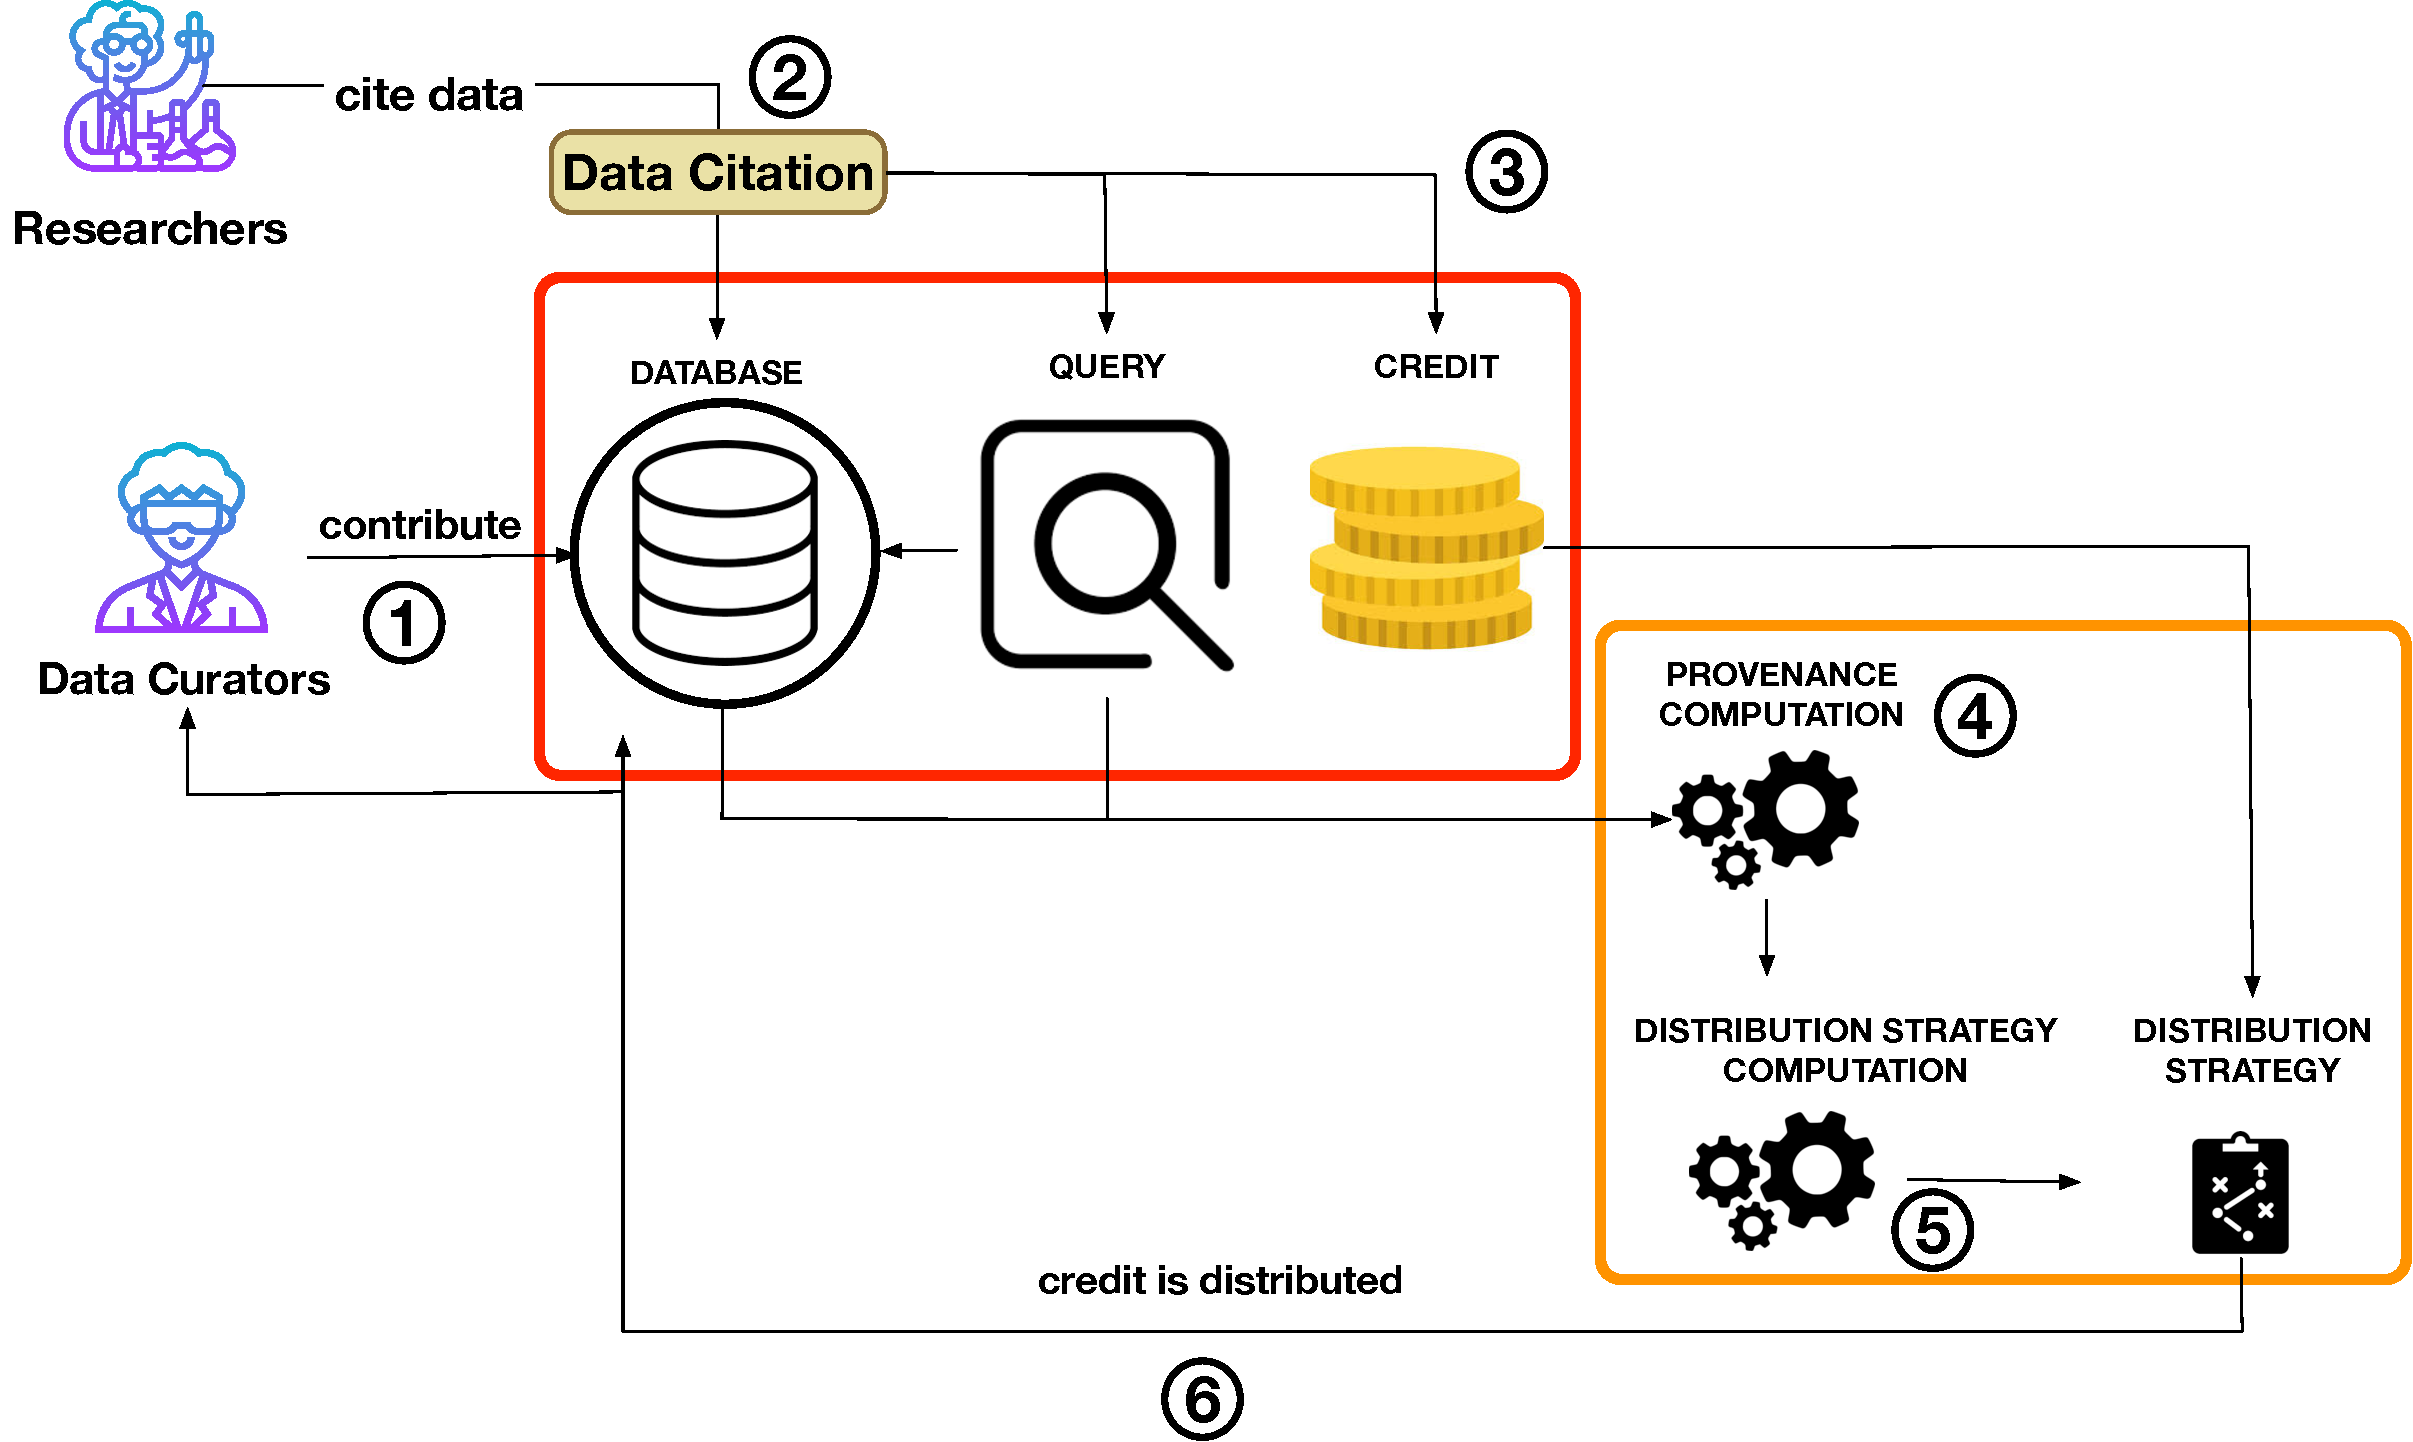
\includegraphics[width=.85\textwidth]{figures/overview}
    \caption{Overview of the credit distribution pipeline.}
    \label{fig:system_overview}
\end{figure}

In Figure \ref{fig:system_overview}, we represent the DCD process:
\begin{description}
	\item[Step 1] The Data Curators are scientist and experts that contribute to the information contained in a scientific database. 
	\item[Step 2] Other researchers use these data in their research. To do so, they use data citation, and thus a query, to identify data in the database.
	\item[Step 3] The citation of data inside the context of a paper generates some credit, that represents the impact of the used data in the research of the paper. The credit is represented as a real value $k \in \mathbb{R}_{>0}$. Without loss of generality, we consider this value as already given.
	\item[Step 4] Given the database instance $I$ and the query $Q$, it is possible to compute the \emph{data provenance} of $Q(I)$. The provenance of $Q(I)$ is a form of metadata that describes the generation process undertaken by $Q$, and the data used in $I$ to generate the output~\citep{CheneyProvSurvey}. Many different notions of provenance have been proposed in the literature for data in database management systems~\citep{lineageCui, WhyProvBuneman, howProvenanceGreen, dosso2020prov}, describing different kinds of relationships between data in the input and the output of a query. As reported in \citep{CheneyProvSurvey}, these provenances, beyond the intrinsic information on how queries work, have been used in several applications, as the study of annotation propagation and view update. In this paper we consider three type of provenance: lineage, why-provenance and how-provenance.
	\item[Step 5] The provenance is the input of the CDC problem, whose aim is the computation of the \emph{Credit Distribution Strategy} (CDS, also referred only as Distribution Strategy, DS). The CDS is a function that distributes $k$ to the data in the input database $I$. 
	CDS functions are to be defined on the basis of citation policies decided at the database administration level or, even better, at the domain community level. 
	Certainly, we are in a one-solution-does-not-fit-all scenario, but CDS can be defined with great variability and flexibility, thus allowing for ample customization. 
	In this paper we describe CDS based on data provenance, and they are therefore closely related to the kind of provenance computed in step 4. In this work we describe three CDS, each based on one of the three considered provenances.
	\item[Step 6] Once the CDS is computed, it is then used to distribute the given credit $k$ to the parts of the database that are responsible for the generation of $Q(I)$. Transitively, this credit is also divided and given to the corresponding authors of those data.
\end{description}

In this paper we expand the work already discussed in our paper \citep{dosso2020data}, where we first asked how to correctly reward data and data curators that are usually left without credit from the current citation systems.
In that paper we first defined the problem of DCD in relational databases (Definition \ref{def:CDT}) and we proposed the possibility to solve the problem by using \emph{lineage}, a form of \emph{data provenance} (Definition \ref{def:lineage_ds}), to define a distribution strategy.
The lineage of a tuple $t$ in the output $Q(I)$ is defined as the set of all and only the tuples in the database instance $I$ that are ``relevant'' to the production of $t$, that is the tuple that are used by $Q$ in the production of $t$. 
The lineage-based strategy equally redistributes the credit $k$ to the tuples in the lineage set, thus each tuple receives credit $k/|L_t|$, where $L_t$ is the lineage set of $t$. 

One may argue that this may not be the perfect solution to the problem, since lineage only tells the relevant tuple used to produce the output. It does not convey any information about their role or importance in the query.
Therefore, one may instead desire to give more credit to the tuples that are more relevant or essential to the production of the output, i.e. those tuples that, if removed, would prevent the output tuple to appear in the final result, or those tuples that are used in more than one operation by the query. 

Therefore, in this paper, we expand the research done in \citep{dosso2020data} by proposing new Distribution Strategies, based on other forms of data provenance. 
Namely, why-provenance~\citep{WhyProvBuneman} and how-provenance~\cite{howProvenanceGreen}. 
We compare them also with the lineage-based one to highlight their differences and how one may be preferred instead of another. 
In particular, we show that why-provenance and how-provenance are more sensitive to the role of a tuple in a query (depending on how many times the tuple is used or how it is used). 
The DS based on why-provenance rewards more the tuples that are essential to the production of a tuple.
The DS based on how-provenance also takes into consideration in how many different ways a tuple is used, presenting an even higher level of sensibility. 

For our experiments we use a well-known curated database, the IUPHAR/BPS\footnote{International Union of Basic and Clinical Pharmacology/British Pharmacology Society} Guide to Pharmacology~\citep{iuphar2018}, also known as GtoPdb\footnote{\url{https://www.guidetopharmacology.org/}}, which contains expertly curated information about diseases, drugs, cellular drug targets and their mechanisms of action.
We chose GtoPdb for two main reasons: (i) it is a widely-used and valuable curated relational database, (ii) many papers in the literature use and cite its data (i.e., families, ligands, and receptors). 
Real queries used in papers can therefore be seen as data citations which, in turn, can be used to assign data credit.

We perform three sets of experiments. In the first one, real queries are extracted from papers published in the British Journal of Pharmacology (BJP), that represent data citations to GtoPdb, and are used to distribute credit in the database using three different DS, based on the three forms of provenance considered. 
We show how, given the peculiar nature of the queries, the three distributions do not present particular differences in this context and why this is the reason. 
In the second and third sets of experiments we show how, using more complex queries, it is possible to see differences, brought forth by the different distributions deriving from the provenance used, and how the more complex the provenance used, the more sensible to the role of the tuples in the production of $t$ the distributions become.


Our paper \emph{contributes} to the following:
\begin{itemize}
    \item Defining new form of Distribution Strategies for the problem of Data Credit Distribution, based on why-provenance and how-provenance;
    \item In-depth analysis of the effects of credit distribution over real-world curated data and the of the differences between the three Distribution Strategies based on the forms of provenance deployed.
\end{itemize}

\paragraph{\textbf{Outline}} The rest of paper is organized as follows:
Section \ref{sec:related} presents the related works; Section \ref{section:use_case} describes the use case we adopted; section \ref{section:preliminaries} briefly presents the provenances used in the paper; Section \ref{section:distribution_strategies} describes the problem of DCD and the new DS developed in this paper; in Section \ref{sec:experiments} we present the evaluation of our approach. Finally, Section \ref{section:conclusions} presents our conclusions and potential future work.

%############


 
